% *********************************************************************
% © 2026 Jeremy Sylvestre
%
% Permission is granted to copy, distribute and/or modify this document
% under the terms of the GNU Free Documentation License, Version 1.3 or
% any later version published by the Free Software Foundation; with no
% Invariant Sections, no Front-Cover Texts, and no Back-Cover Texts. A
% copy of the license is included in the appendix entitled “GNU Free
% Documentation License” that appears in the output document of this
% PreTeXt source code. All trademarks™ are the registered® marks of
% their respective owners.
%
% *********************************************************************
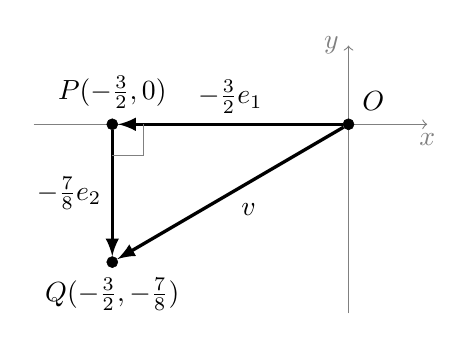
\begin{tikzpicture}[
	point/.style={circle,draw,very thin,fill,inner sep=0pt,minimum size=4pt},
	vector/.style={-latex,very thick},
	scale=2
]
	\draw[gray,->] (-2,0) to (0.5,0) node[below] {$x$};
	\draw[gray,->] (0,-1.2) to (0,0.5) node[left] {$y$};

	\node[point] at (0,0) (o) [label=above right:$O$] {};
	\node[point] at (-1.5,0) (p) [label=above:{$P(-\frac{3}{2},0)$}] {};
	\draw[vector] (o) to node[above] {$- \frac{3}{2} \uvec{e}_1$} (p);
	\node[point] at (-1.5,-0.875) (q) [label=below:{$Q(-\frac{3}{2},-\frac{7}{8})$}] {};
	\draw[vector] (p) to node[left] {$- \frac{7}{8} \uvec{e}_2$} (q);
	\draw[vector] (o) to node[below right] {$\uvec{v}$} (q);

	% perp symbol
	\draw[thin,gray] (-1.3,0) to (-1.3,-0.2) to (-1.5,-0.2);

\end{tikzpicture}
